\documentclass[11pt]{article}
\usepackage{algorithm2e}
\usepackage[italian]{babel}
\usepackage[document]{ragged2e}
\usepackage{amsfonts, amssymb, amsmath}
\usepackage{cancel}
\usepackage{float}
\usepackage{mathtools}
\usepackage[margin=3cm]{geometry}

\tolerance=1
\emergencystretch=\maxdimen
\hyphenpenalty=10000
\hbadness=10000

\begin{document}
\begin{titlepage}
    \begin{center}
        \vspace*{1.5cm}
            
        \Huge
        \textbf{Tweet Analysis}
            
        \vspace{0.3cm}
        \LARGE
        Sprint 2\\[0.2em]
        \Large
        3 novembre 2022 -- 16 novembre 2022

        \vspace{1.5cm}
          
        \begin{minipage}[t]{0.47\textwidth}
            \begin{center}
                \parbox{50mm}{\centering\large {\bf Cheikh Ibrahim $\cdot$ Zaid} \\[0.2em] PO Operativo \\[0.3em] Matricola: \texttt{0000974909}}\\[2em]
                \parbox{50mm}{\centering\large {\bf Lee $\cdot$ Qun Hao Henry} \\[0.2em] Developer \\[0.3em] Matricola: \texttt{0000990259}}
            \end{center}
		\end{minipage}
		\hfill
		\begin{minipage}[t]{0.47\textwidth}\raggedleft
            \begin{center}
                \parbox{50mm}{\centering\large {\bf Xia $\cdot$ Tian Cheng} \\[0.2em] Scrum master \\[0.3em] Matricola: \texttt{0000975129}}\\[2em]
                \parbox{50mm}{\centering\large {\bf Paris $\cdot$ Manuel} \\[0.2em] Developer \\[0.3em] Matricola: \texttt{0000997526}}
            \end{center}
		\end{minipage}  
            
        \vspace{6cm}
            
        Anno accademico\\
        $2022 - 2023$
            
        \vspace{0.8cm}
            
            
        \Large
        Corso di Ingegneria del Software\\
        Alma Mater Studiorum $\cdot$ Università di Bologna\\
            
    \end{center}
\end{titlepage}
\pagebreak


\section*{Sprint goal}
\justify
Lo sprint è stato dedicato alla conclusione dell'epica riguardante la visualizzazione e l'analisi dei tweet.\\
Nello specifico, sono state implementate le seguenti feature:
\begin{itemize}
    \item Ricerca di tweet per intervallo temporale (richiesto dal cliente allo sprint review precedente)
    \item Ricerca di un determinato numero di tweet con una singola ricerca (richiesto dal cliente allo sprint review precedente)
    \item Ricerca di tweet per parola chiave
    \item Mappa per visualizzare la posizione dei tweet con geolocalizzazione
    \item Raccolta di tweet in tempo reale
\end{itemize}


\begin{figure}[H]
    \centering
    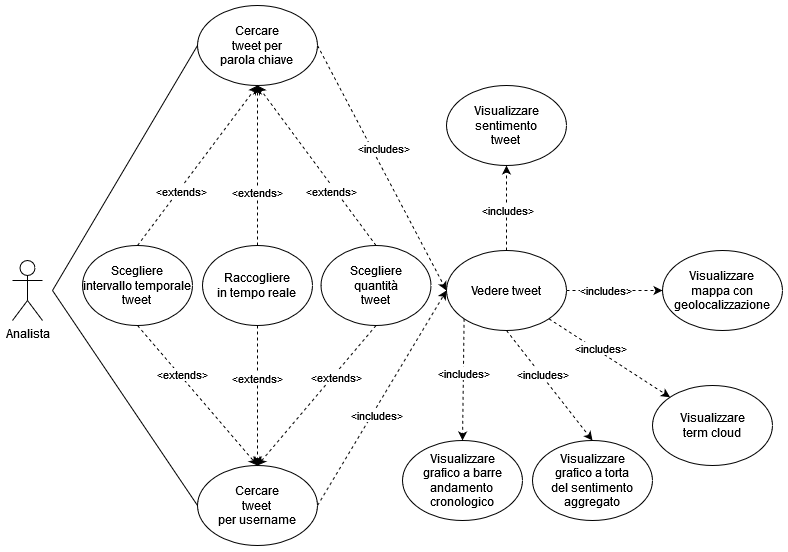
\includegraphics[width=12cm]{./img/usecase.png}
    \caption{Use case previsto per lo sprint 2}
\end{figure}

\newpage
\section*{Esito sprint}
Lo sprint è terminato con la conclusione di tutte le user stories pianificate.\\
Il lavoro si è svolto in linea con l'andamento ideale dei punti. 
Si è osservato una leggera sovrastima delle user stories che ha portato alla conclusione anticipata (di un giorno) dello sprint.\\
Le ore di lavoro sono state distribute in periodi di maggiore produttività e periodi di sviluppo più lento, ma comunque è stato rispettato il monte ore dello sprint.
\begin{figure}[H]
    \centering
    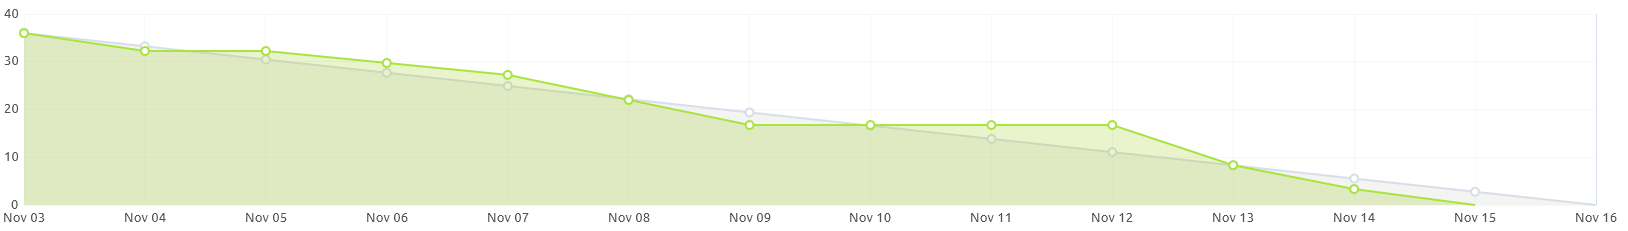
\includegraphics[width=\textwidth]{./img/burndown.png}
    \caption{Burndown generato da Taiga}
\end{figure}

\begin{figure}[H]
    \centering
    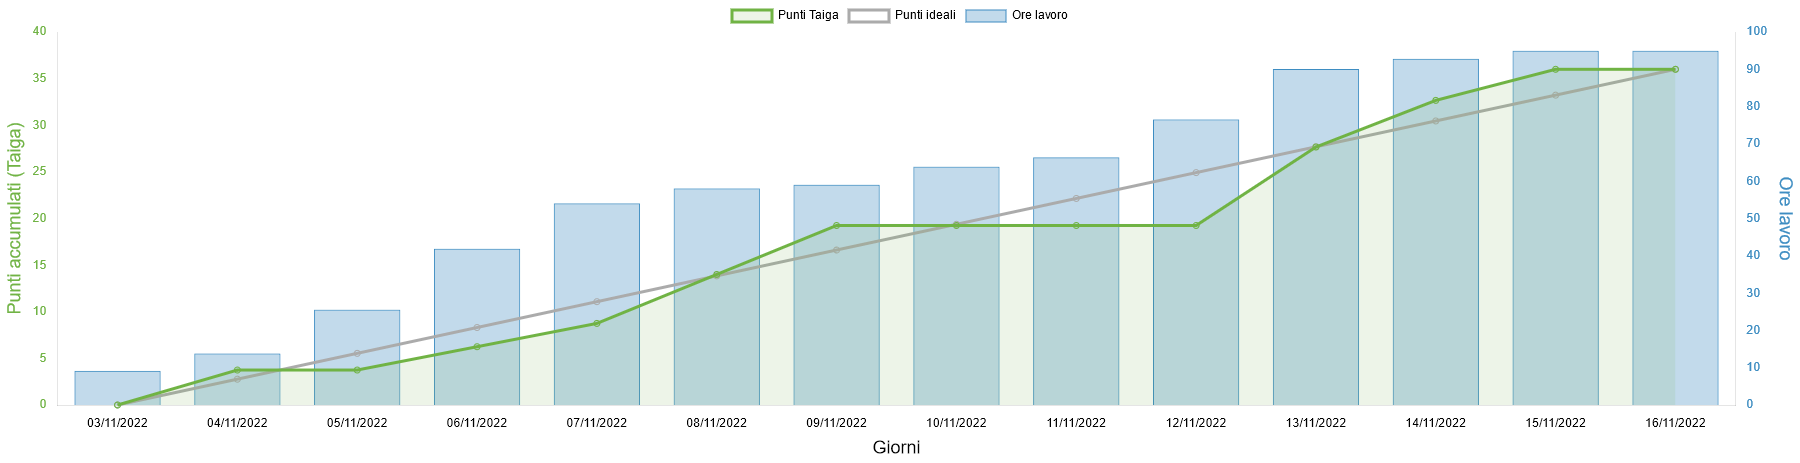
\includegraphics[width=\textwidth]{./img/worktime.png}
    \caption{Progresso dei punti (asse a sinistra) e ore di lavoro (asse a destra)}
\end{figure}

\section*{Sprint review}
Allo sprint review non sono emerse nuove richieste da parte del cliente.

\newpage
\section*{Retrospettiva}
\subsection*{Pre-retrospettiva}
Alla pre-retrospettiva effettuata a metà sprint, sono emerse le seguenti problematiche:
\begin{itemize}
    \item Mancanza di test adeguati per il frontend
    \item Le user stories sono state sovrastimate
\end{itemize}
\begin{figure}[H]
    \centering
    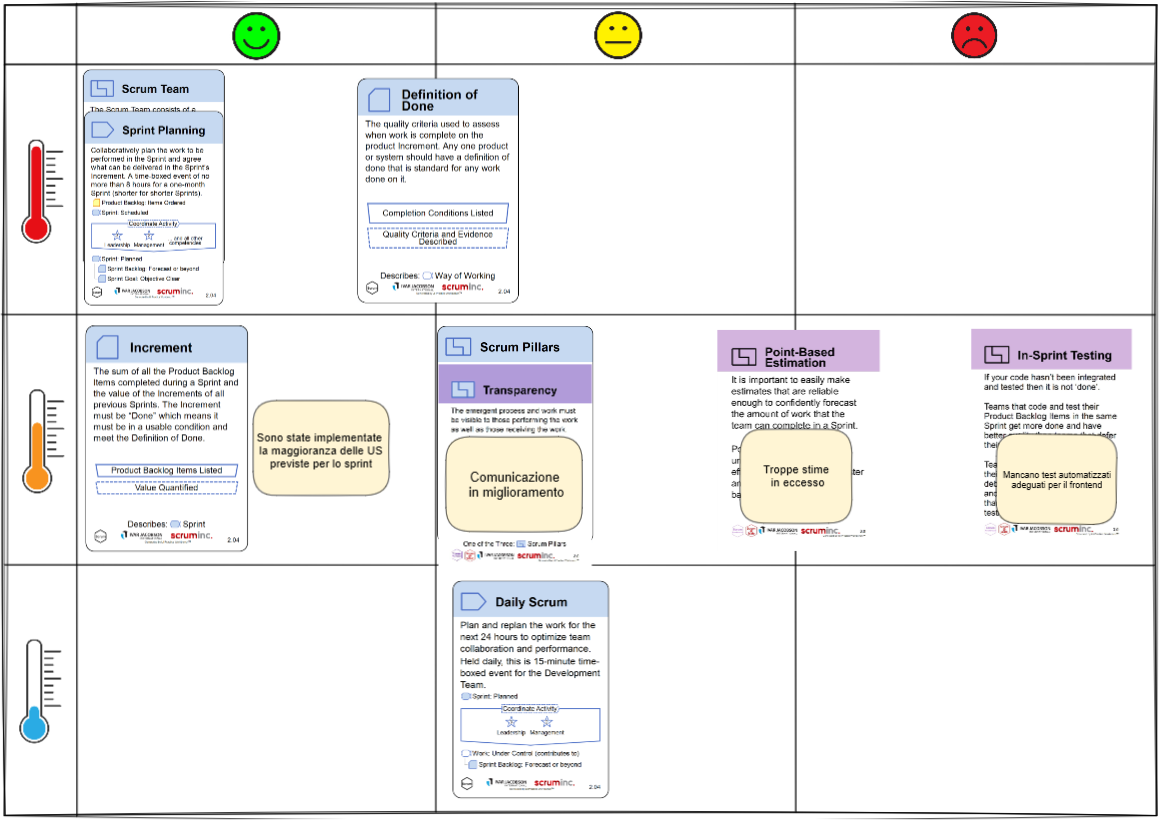
\includegraphics[width=12cm]{./img/preretrospettiva.png}
    \caption{Carte Essence giocate alla pre-retrospettiva}
\end{figure}

\subsection*{Retrospettiva}
Alla retrospettiva di fine sprint sono state confermate le problematiche della pre-retrospettiva.



\end{document}

